\chapter{Results}
\label{chap:results}

In this chapter, we present the main results of our dark siren cosmology analysis using brightness-ranked subsets of the \texttt{GLADE+} galaxy catalog. We evaluate the impact of applying magnitude cuts on the galaxy sample, compare the resulting \ac{LOS} redshift priors, and show how these choices affect the posterior distribution of the Hubble constant $H_0$. We also assess the precision-bias trade-off associated with aggressive catalog cuts.

\section{LOS Redshit Prior}
The first step in our cosmological inference is computing the \ac{LOS} redshift prior $p(z | \Omega, \Lambda, s, I)$ for each \ac{GW} event and sky pixel $\Omega$. This prior combines the redshift distribution of galaxies in the \texttt{GLADE+} catalog with an analytic model for the out-of-catalog population, as described in Chapter~\ref{chap:methodology}.

To test the impact of catalog completeness, we apply successive cuts to the galaxy catalog by selecting only the brightest $XX\%$ of galaxies in $K$-band luminosity, forming subsets labeled \texttt{GLADEPXX}. This process shifts the effective magnitude threshold upward, reducing the number of galaxies but improving the catalog's completeness above the cut.

Figure~\ref{fig:los_prior_gw170809} shows the LOS redshift prior for the event GW170809 under different catalog cuts. Bright galaxy subsets (e.g., \texttt{GLADEP20}) result in sharper redshift distributions and reduce the weight of the out-of-catalog term. Notably, these priors maintain consistency in shape, indicating that bright galaxies are reliable tracers of large-scale structure. The application of a brightness cut significantly modifies the \ac{LOS} redshift distribution. Specifically, the bright galaxy subsets yield an amplified redshift prior at higher distances, effectively extending the reach of the catalogue, somewhat mitigating the incompleteness issues that arise at deeper redshifts.

\begin{figure}[ht]
    \centering
    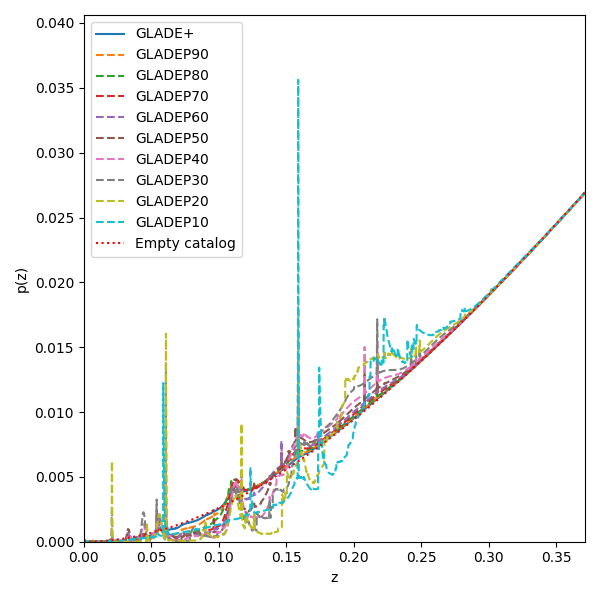
\includegraphics[width=0.7\textwidth]{figures/GW170809_zprior.png}
    \caption[LOS redshift prior for GW170809 for different brightness-ranked \texttt{GLADE} subsets]{LOS redshift prior for GW170809 for different brightness-ranked \texttt{GLADE} subsets. The full \texttt{GLADE+} catalog (solid blue) is compared to the different subsets. Applying a brightness cut amplifies the prior at higher distances, extending the effective reach of the catalog and partially mitigating incompleteness at greater redshifts.}
    \label{fig:los_prior_gw170809}
\end{figure}

\section{$H_0$ Posterior}

With \ac{LOS} priors in hand, we compute the posterior distribution for the Hubble constant $H_0$ by combining the GW posterior $p(d_L, \Omega | \text{GW})$ with the redshift prior $p(z | \Omega, \Lambda, s, I)$. This is done using the \texttt{gwcosmo} pipeline for each event.

Figure~\ref{fig:h0_gw170809} shows the resulting $H_0$ posteriors for GW170809 under various catalog cuts. As the catalog is restricted to brighter galaxies, the $H_0$ posterior becomes increasingly narrow. For example, GLADEP20 yields a visibly tighter posterior compared to the full GLADE+, with minimal shift in the median. However, the most aggressive cut (GLADEP10) introduces broader tails, likely due to insufficient galaxy sampling in the localization volume.

\begin{figure}[ht]
    \centering
    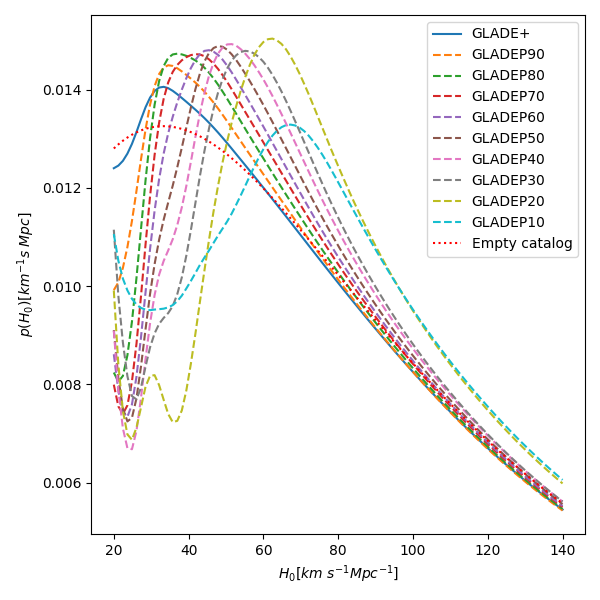
\includegraphics[width=0.7\textwidth]{figures/GW170809_H0.png}
    \caption[$H_0$ posterior distributions for GW170809 using full and brightness-cut galaxy catalogs.]{$H_0$ posterior distributions for GW170809 using full and brightness-cut galaxy catalogs. \texttt{GLADEP20} yields the tightest credible interval. \texttt{GLADEP10} suffers from sparse sampling.}
    \label{fig:h0_gw170809}
\end{figure}

We repeat this procedure for a subset of \ac{BBH} events from \ac{GWTC} that meet our selection criteria. Figure~\ref{fig:h0_cumulative} shows the combined $H_0$ posterior from the selected dark siren events using the full \texttt{GLADE+} catalog and the different subsets.

Table~\ref{tab:h0_stats} summarizes the $H_0$ posteriors for all cuts. The uncertainty is minimized around the \texttt{GLADEP20} subset, showing 30-40\% tighter contraints, while median values shift towards a higher value. For less extreme cuts, the median values doesn't show a huge shift. This suggests that moderate brightness cuts improve precision without introducing systematic bias.

\begin{figure}[ht]
    \centering
    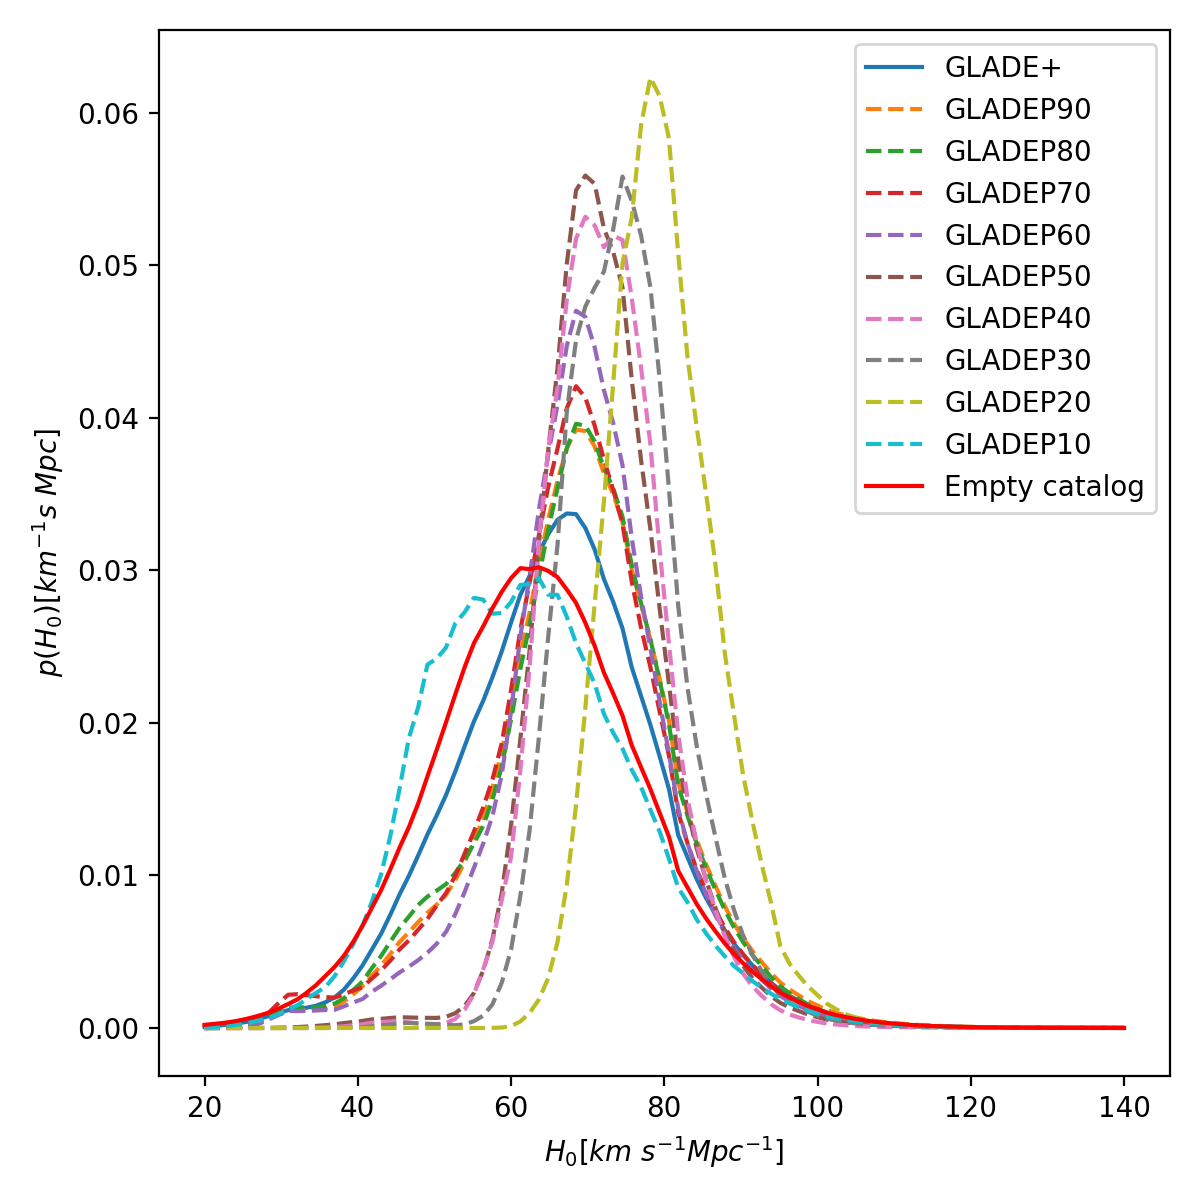
\includegraphics[width=0.7\textwidth]{figures/percentile_full_dict.png}
    \caption[Cumulative $H_0$ posterior from the slected dark siren events using full \texttt{GLADE+} and the different subsets.]{Cumulative $H_0$ posterior from the slected dark siren events using full \texttt{GLADE+} (blue) and the different subsets (dashed lines). The brightness-weighted catalog yields a tighter constraint without a significant shift.}
    \label{fig:h0_cumulative}
\end{figure}

\begin{table}
    \centering
    \caption[$H_0$ MAP values with $68\%$ confidence ranges, alongside the maximum magnitude limits for \texttt{GLADE+} and the different subsets.]{Maximum {\em a posteriori} probabilities with $68\%$ confidence ranges of the $H_0$ posterior distributions alongside the maximum magnitude limits for the different percentiles of the GLADE+ galaxy catalogue.}
    \begin{tabular}{c c c }
    \hline
        \textbf{Catalogue} & \textbf{$M_{K, max}$} & \textbf{$H_0~[km~s^{-1}Mpc^{-1}]$} \\ \hline
        \texttt{GLADE+} & -19.00 & $67.87^{+8.97}_{-10.29}$ \\
        \texttt{GLADEP90} & -23.07 & $68.94^{+9.24}_{-7.55}$ \\
        \texttt{GLADEP80} & -23.62 & $68.93^{+9.25}_{-7.57}$ \\
        \texttt{GLADEP70} & -23.94 & $68.63^{+8.61}_{-7.42}$ \\
        \texttt{GLADEP60} & -24.19 & $68.85^{+7.72}_{-6.43}$ \\
        \texttt{GLADEP50} & -24.14  & $70.05^{+6.12}_{-5.20}$ \\
        \texttt{GLADEP40} & -24.63 & $69.94^{+7.46}_{-3.88}$ \\
        \texttt{GLADEP30} & -24.87 & $74.70^{+4.69}_{-6.58}$ \\
        \texttt{GLADEP20} & -25.15 & $78.28^{+5.53}_{-4.95}$ \\
        \texttt{GLADEP10} & -25.53 & $63.46^{+6.39}_{-14.37}$ \\ \hline
    \end{tabular}
    \label{tab:h0_stats}
\end{table}

\section{Cost–benefit trade-off}
We observe that precision improves with increasing brightness until an optimum is reached (near \texttt{GLADEP20}). Beyond this point, the posterior widens again due to under-sampling. This defines a practical limit for catalog pruning. In real applications, the exact optimum may depend on event SNR, catalog completeness, and the merger rate model.

Our results suggest that targeting the brightest galaxies in a well-characterized catalog can substantially improve the statistical precision of $H_0$ constraints from dark sirens. This approach complements other efforts to mitigate catalog incompleteness, including joint inference with galaxy clustering and population-informed redshift estimation.